\section{Design}
\label{sec:Design}

\subsection{Database Design} 
\paragraph{}The Bmob online database was chosen for the database management system (DBMS) for both the Android application and the web interface because it is a free and open source product that supports the applications required use-cases. 
\par Bmob cloud storage service platform is a secure and flexible background management system. In addition to the security processing on the server deployment, the Bmob cloud storage service platform adopts a multi-tenant virtual isolation mode, that is, any developer's traffic changes or data changes will not affect other developers' applications. It also supports a wide range of data types, including String, Number(including integers and floats), Boolean, Date, File, Geopoint(GPS Position), Array and Object. In this project we will use most of them.
Another reason to choose Bmob is it supports API interface and multi-language SDK, like Android, IOS, REST API, GO and so on. For our project, we will use both REST API and Android API. It can supports various file uploads and storage,including pictures, videos, audio, and documents, but we will mainly use to upload image files in this project, CDN acceleration also makes it faster and more stable.
\par The entity relationship (ER) diagram for the whole project is shown in Figure \ref{ERDiagram}.

\begin{figure}[htb]
\centering
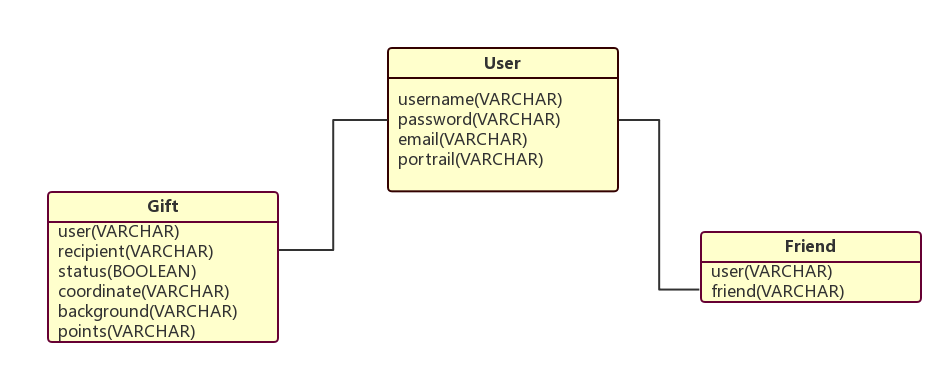
\includegraphics[width=.9\textwidth]{section03/assets/ERDiagram.png}
\caption[Short Caption 2]{\label{ERDiagram}ER Diagram for the project}
\end{figure}

\paragraph{}
All three tables designed for this project are listed in the ER Diagram.
\begin{itemize}
\item The 'User' table will save all the user information. In this table username and email will be unique for each user and this will be verified when users are registered.
\item The 'Friend' table is for saving all friends pairs and both 'user' and 'friend' columns are usernames from 'User' table.
\item The 'Gift' table saves all the gifts information. The 'user' column records the user who sent the gift. The 'recipient' column records the user who will receive the gift. The 'status' column is a boolean type data meaning the gift is found if it is 'true'. The 'coordinate' column is designed to hold the location where the gift was sent. The 'background' column is designed to hold the region picture and the 'points' column is designed to hold the four corners selected by users.
\end{itemize}

\subsection{User Interface Design}
\paragraph{}Following the user interface design principles, like the accessibility, flexibility, consistency and aesthetically pleasing, this user interface is designed to be clear and easy to use. All the parts keep the same color style and try not to use too many colors and fonts so that the user interface is aesthetically pleasing. The main pages are listed below:
\begin{figure}[htb]
\centering
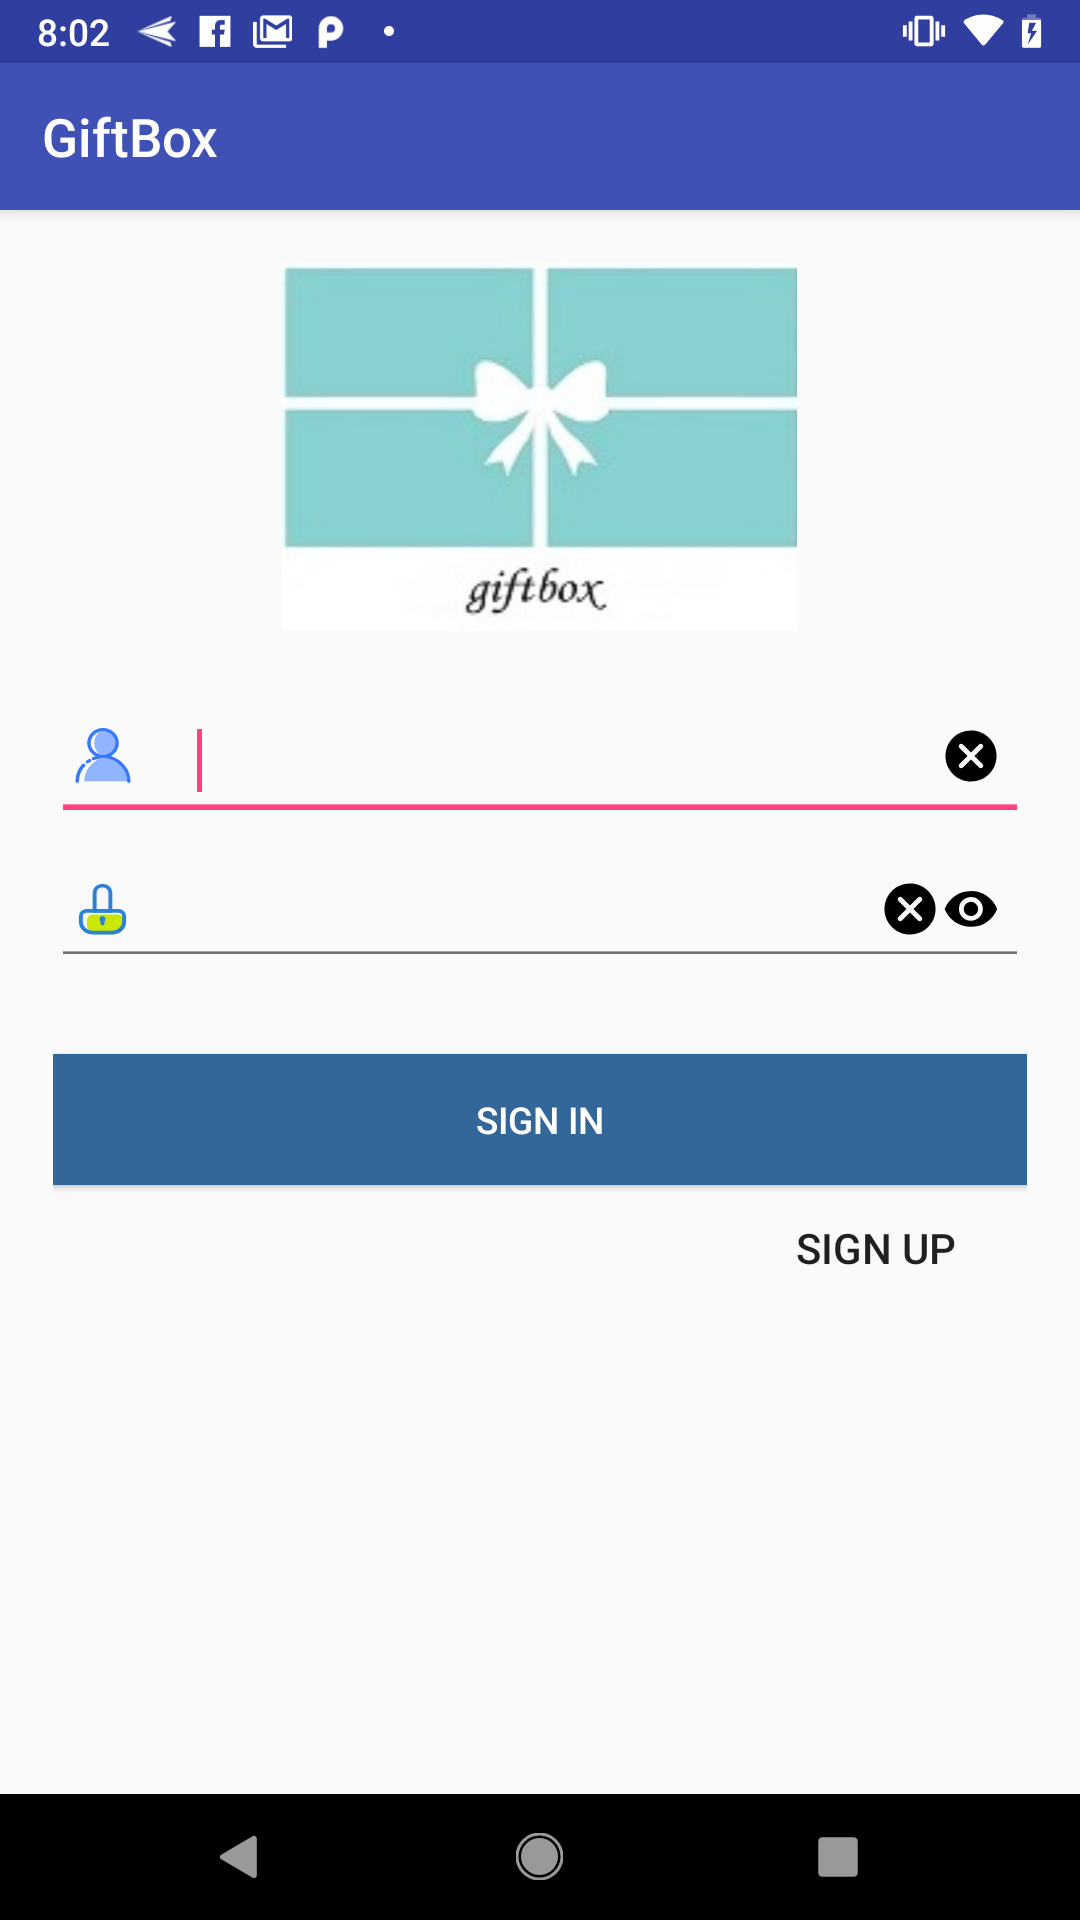
\includegraphics[width=.27\textwidth]{section03/assets/SignIn.png}
\caption[Short Caption 2]{\label{SignInUI}Sign In Page}
\end{figure}
\par The sign in page is shown in Figure \ref{SignInUI}. The logo is designed to show up so that the user will know which application they are using. The user icon and the password icon at the left side of the text field hint the meaning of the two fields to the users. To maintain the compatibility, the delete icon and the eye icon at the right side of the text field used another color because they have different functions. Users can use the delete button to delete the whole string they typed in and view the password in plain text or hidden text. to maintain the forgiveness the 'Log In' button is designed to be big to prevent users from making mistakes. 

\begin{figure}[htb]
\centering
\begin{minipage}[t]{0.27\textwidth}
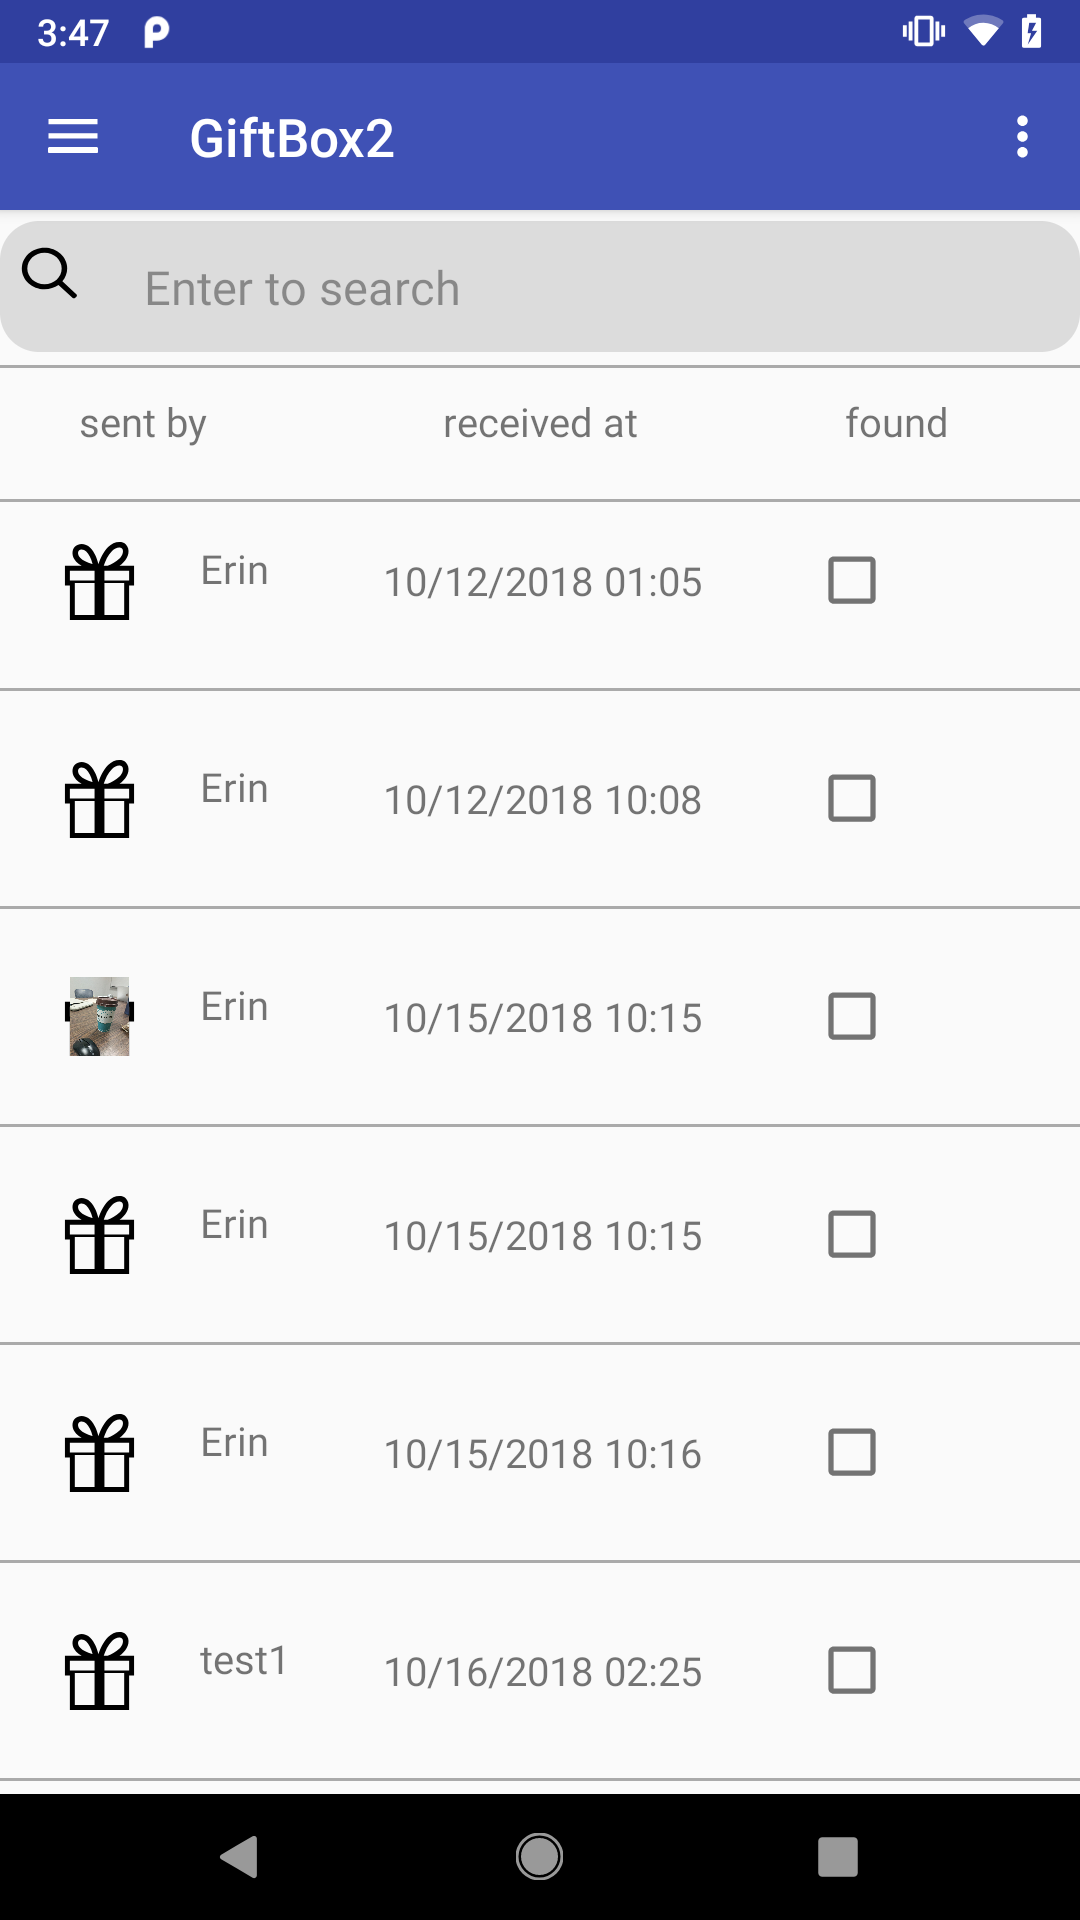
\includegraphics[width=.95\textwidth]{section03/assets/MainPage.png}
\subcaption{\label{GiftsListMainUI}}
\end{minipage}%
\begin{minipage}[t]{0.27\textwidth}
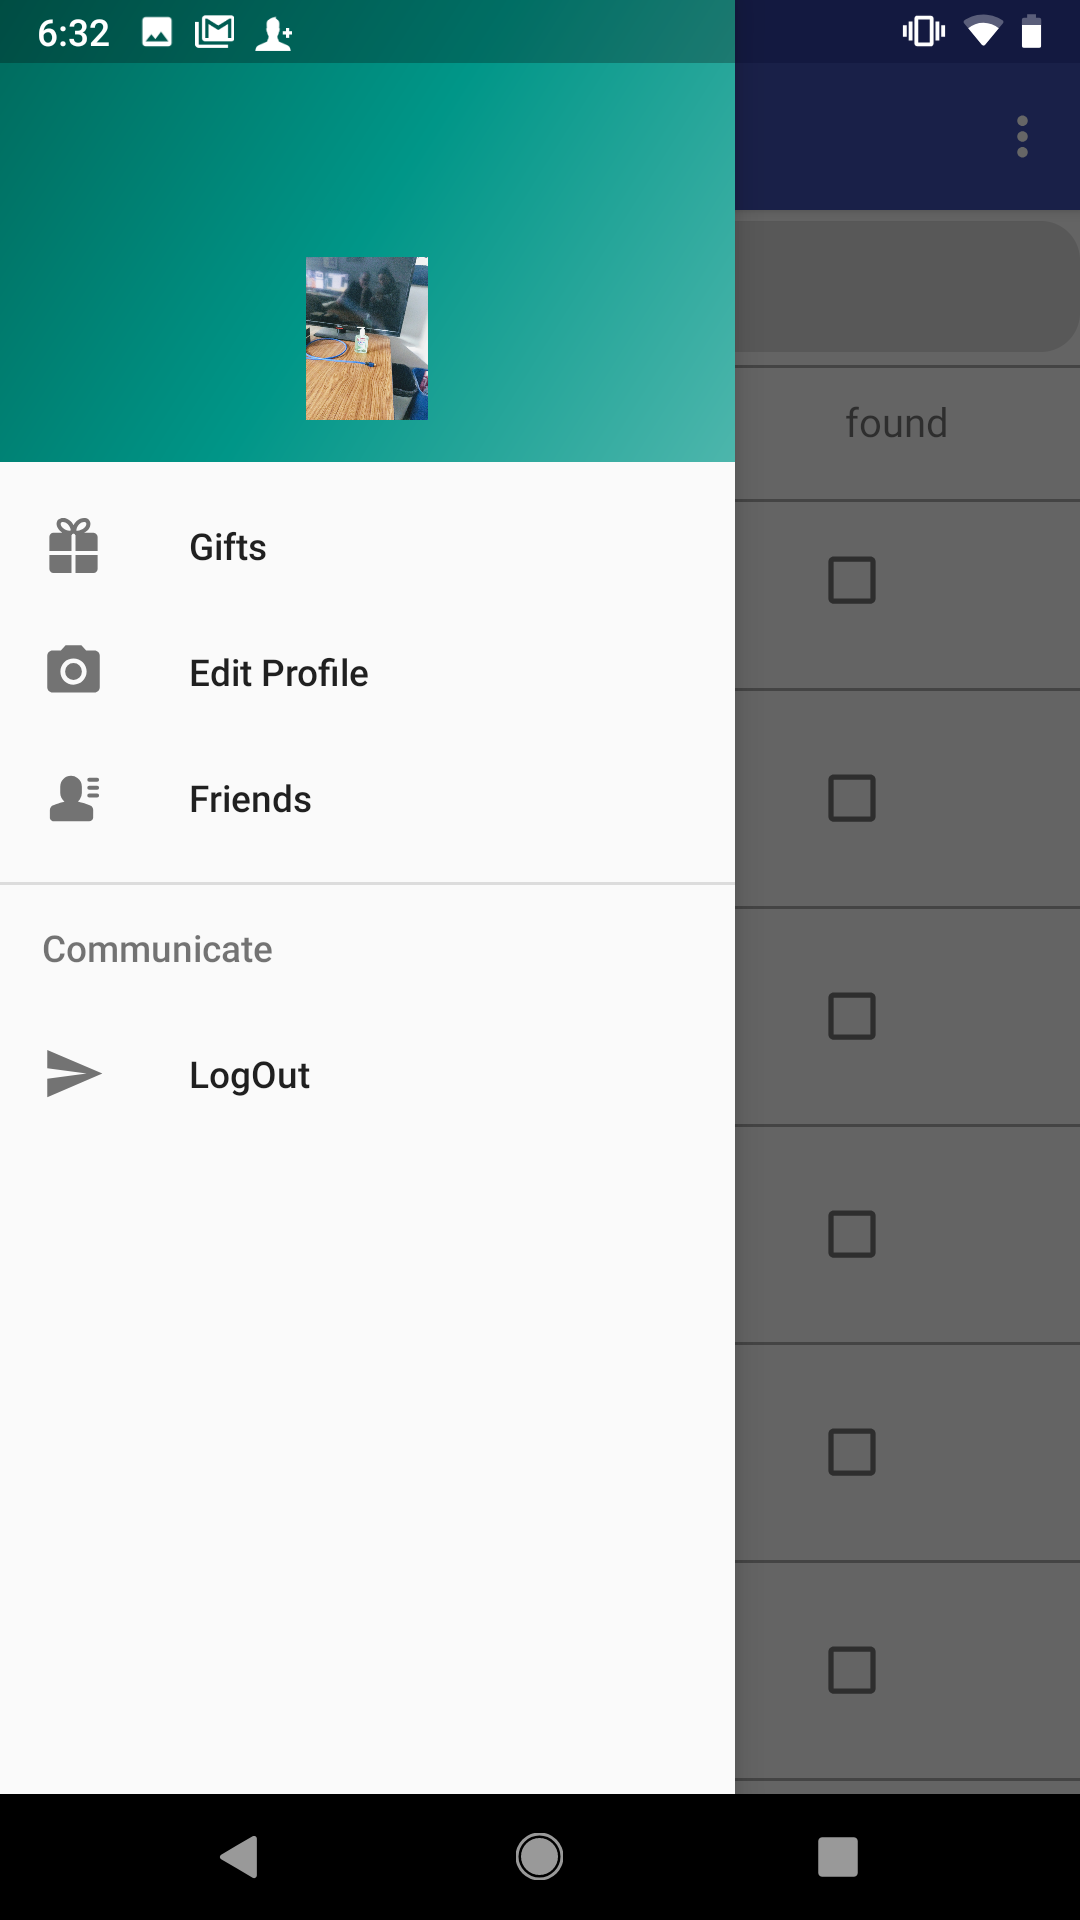
\includegraphics[width=.95\textwidth]{section03/assets/MainPortrait.png}
\subcaption{\label{FunctionsMainUI}}
\end{minipage}%
\caption[Short Caption 2]{\label{MainPageUI}Main Page}
\end{figure}
\par The main page shown in Figure \ref{MainPageUI} will come up after users log in. The Figure \ref{GiftsListMainUI} shows the gifts received by the user. The top search field can searched by username. This page also has titles to tell user the meaning of each column. The gift icon was replaced by user portraits later. The found column shows whether or not the gift is found. If the box is checked that means the gift is found.
\par The top left corner navigation menu will lead users to other functional pages. Users will see their portraits on the top of this page and will be able to change their portraits by clicking on the profile picture. They can also view their gifts list by clicking on the 'Gifts' button, edit their profile by clicking on the 'Edit Profile' button, view their friends list as shown in Figure \ref{FriendsListUI} by clicking on the 'Friends' button and they will be able to log out from the system by clicking on the 'LogOut' button. 

\begin{figure}[htb]
\centering
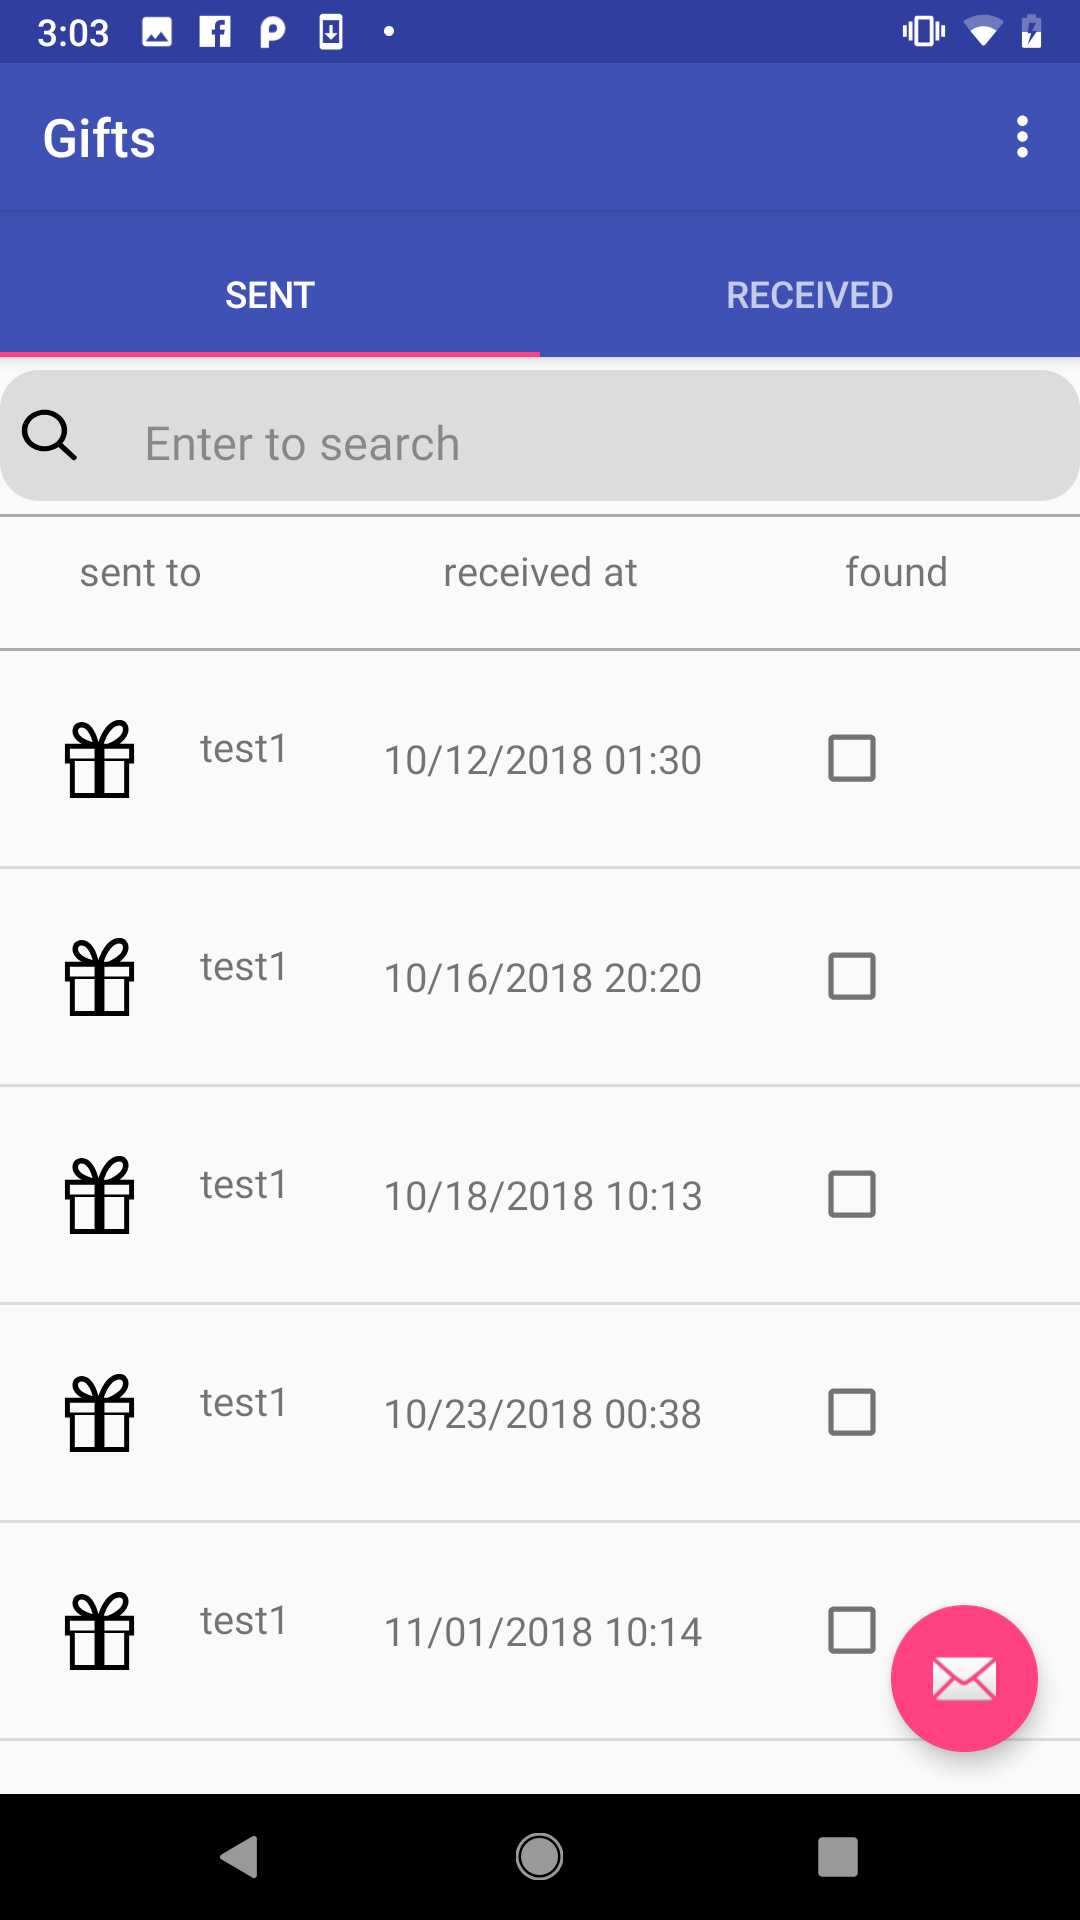
\includegraphics[width=.27\textwidth]{section03/assets/GiftsList.png}
\caption[Short Caption 2]{\label{GiftsListUI}Gifts List Page}
\end{figure}
\par Figure \ref{GiftsListUI}, gifts list page is very similar to the main page's gifts list but in this page users will be able to see not only received gifts but also sent gifts ordered by time stamp. For the sent gifts, users will be able to see if this gift is found or not by clicking on the gift. For the received gifts, they can only view found gifts and begin to find unfound gifts by clicking on the gift. 


\begin{figure}[H]
\centering
\begin{minipage}[t]{0.27\textwidth}
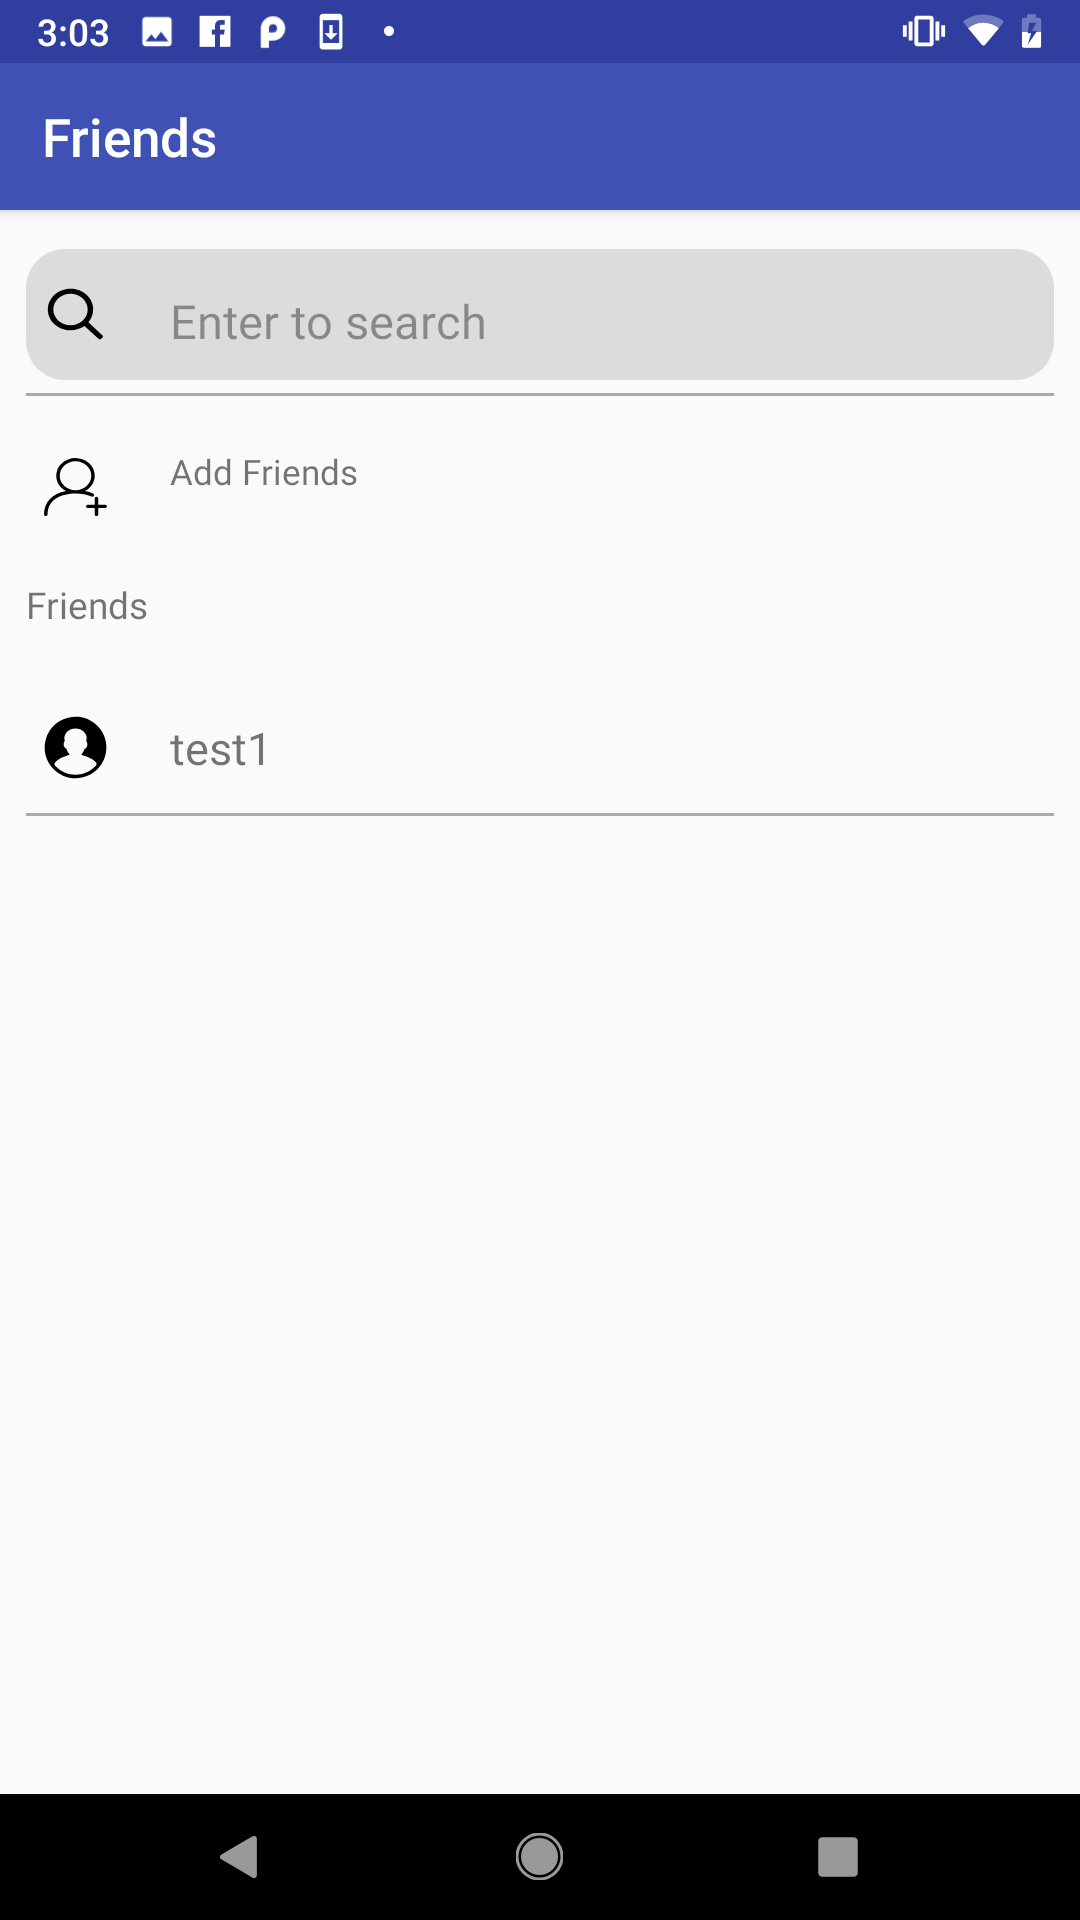
\includegraphics[width=.95\textwidth]{section03/assets/FriendsList.png}
\subcaption{\label{FriendsListUI}}
\end{minipage}%
\begin{minipage}[t]{0.27\textwidth}
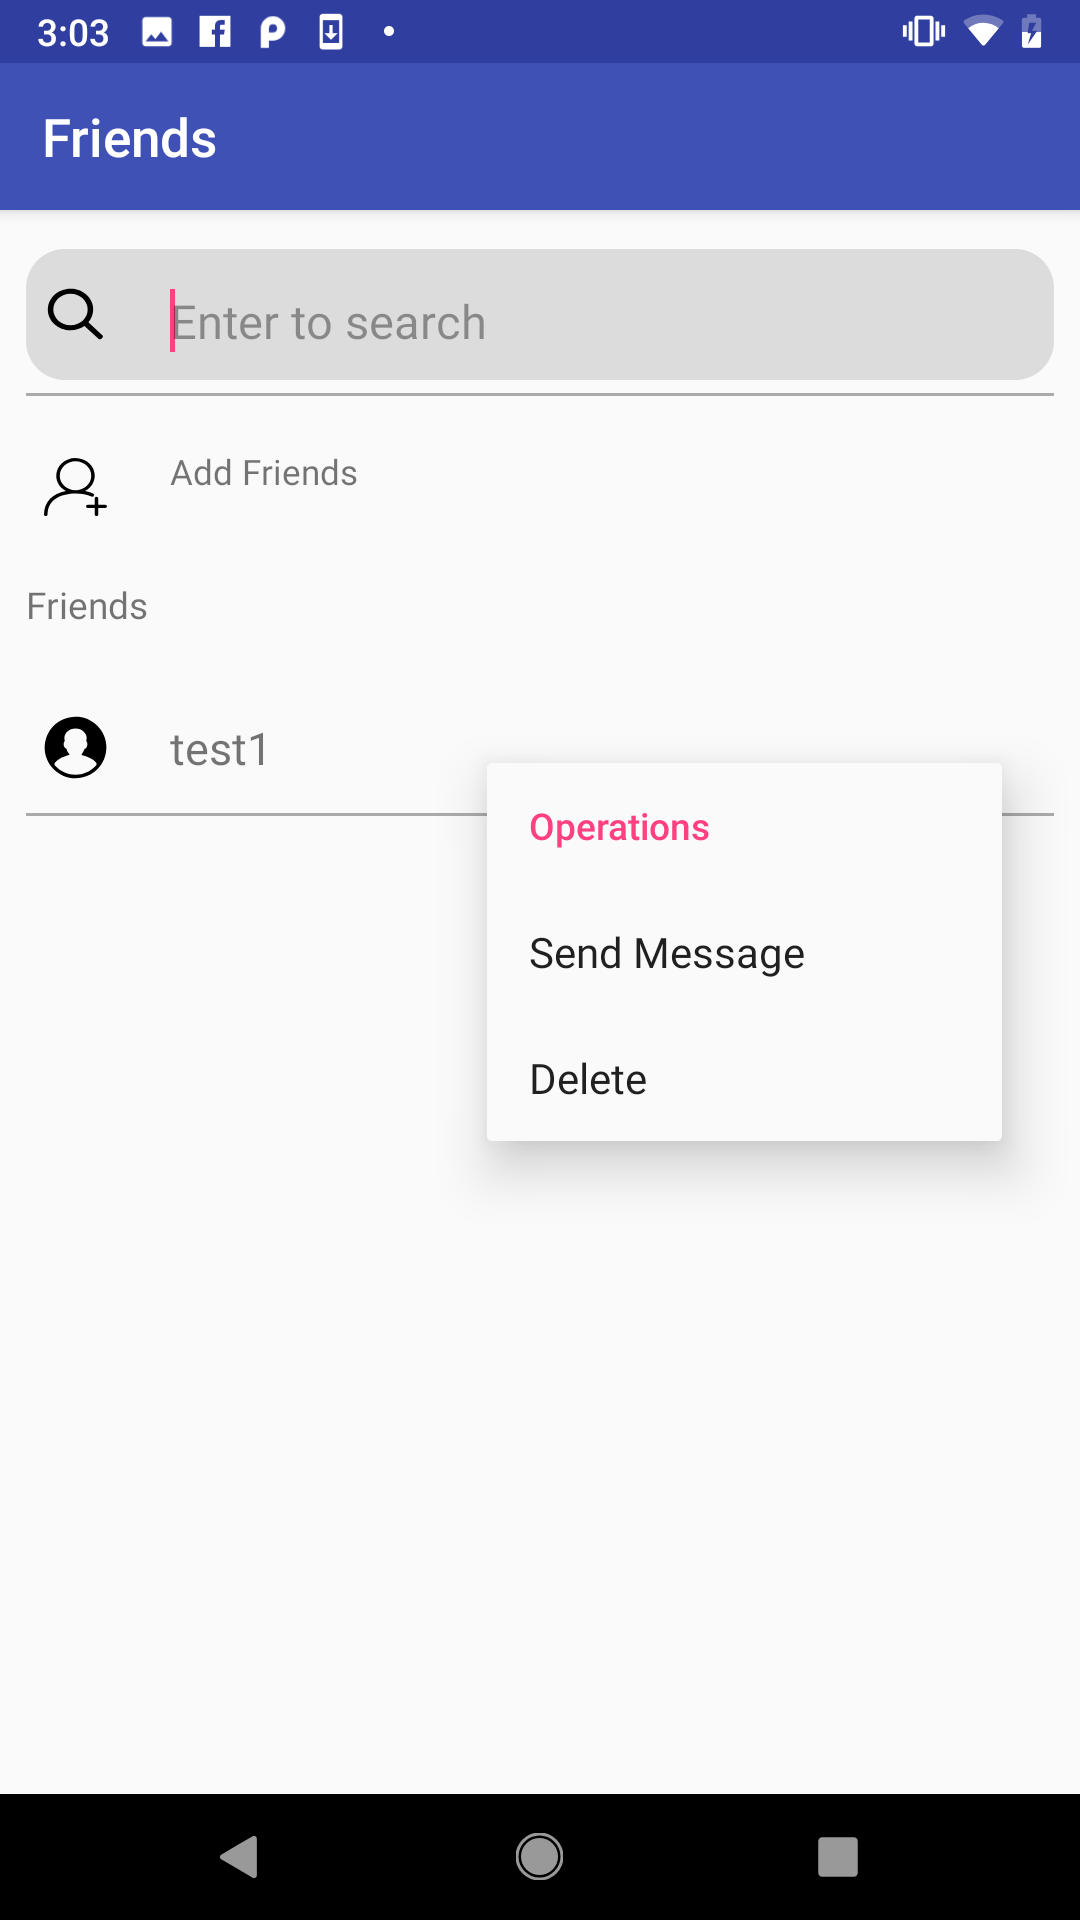
\includegraphics[width=.95\textwidth]{section03/assets/FriendsListAction.png}
\subcaption{\label{FriendsListActionUI}}
\end{minipage}%
\caption[Short Caption 2]{\label{WholeFriendsListUI}Friends List Page}
\end{figure}

\par As shown in Figure \ref{WholeFriendsListUI}, the friends list is another important page for this application. To convenience users, the search field can let users search their friends if their friends list is too long. Users can also add friends by clicking on the 'Add Friends' button. The friends list is shown below. Users can get further functions like 'Send Message' and 'Delete' by a long clicking on friends' names, as shown in Figure \ref{FriendsListActionUI}. 

\begin{figure}[ht]
\centering
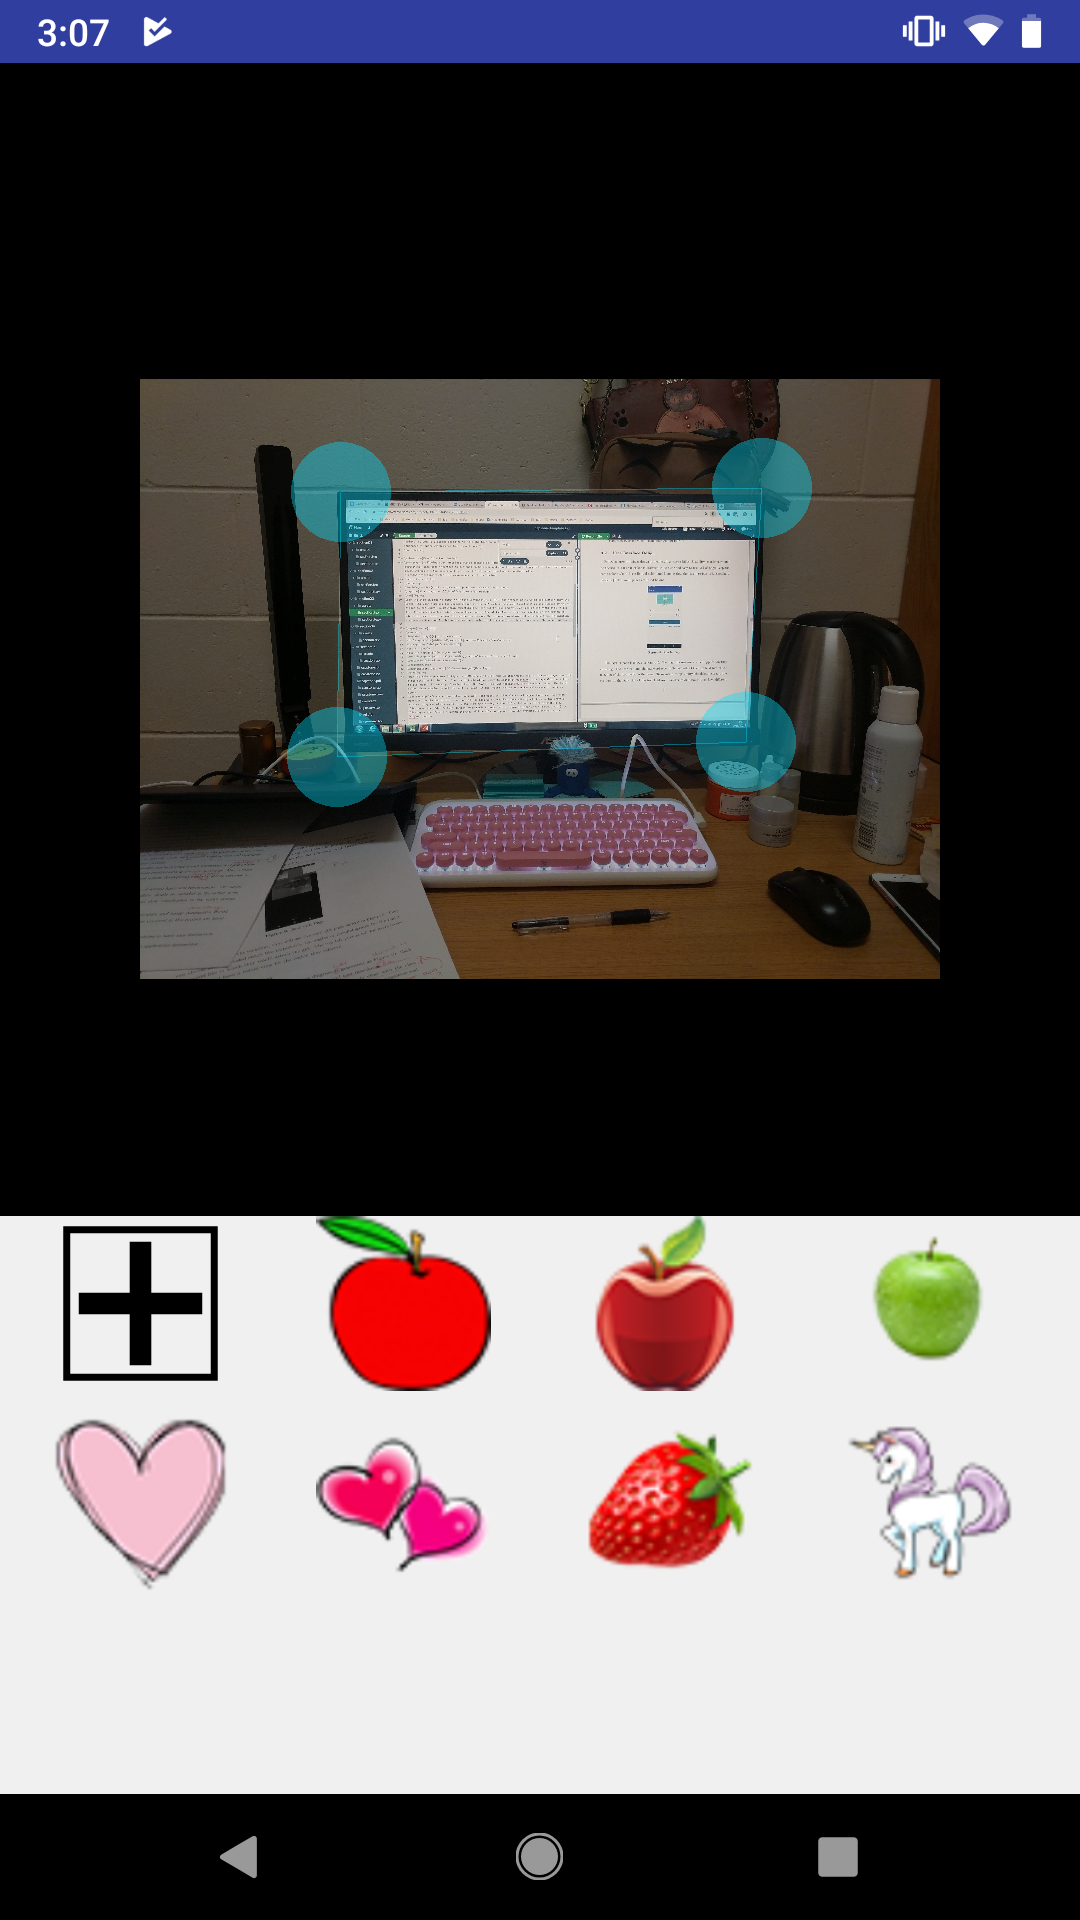
\includegraphics[width=.27\textwidth]{section03/assets/SendGift.png}
\caption[Short Caption 2]{\label{SendGiftUI}Send Gift Page}
\end{figure}
\par After users choose the recipient, they will see the send gift page shown in Figure \ref{SendGiftUI}. They can choose any four sided shape like trapezoids, rectangles or parallelograms for the region they would like in which they would attach the gift. The top left part is left for users to see more details and have a better view for the region they selected.

\subsection{Architecture Design}
\paragraph{}Based on the functional requirements, the class diagram is generated as Figure \ref{ClassDiagram}. Each class corresponds to one or more functional requirements and user interfaces.
\par As we can see, the basic user interaction related class is already clear with the class diagram. So we are just going to explain classes and functions about image recognition and navigation.

\begin{figure}[H]
\centering
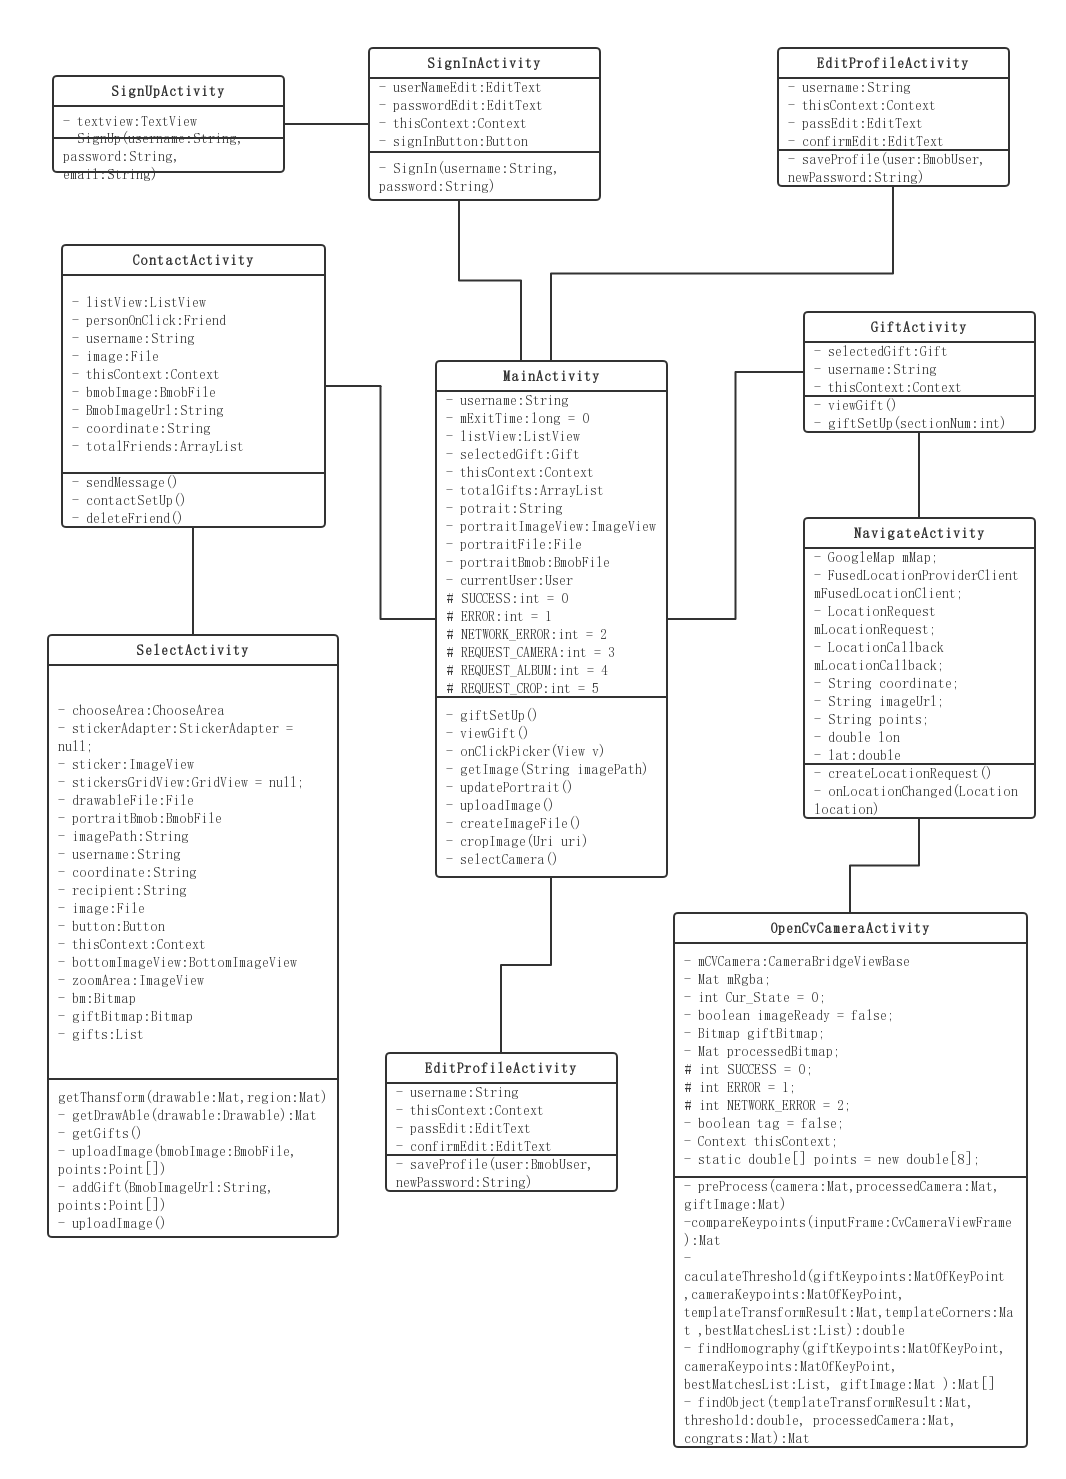
\includegraphics[width=.9\textwidth]{section03/assets/ClassDiagram.png}
\caption[Short Caption 2]{\label{ClassDiagram}Class Diagram}
\end{figure}
\par The 'ContactActivity' is mainly related to the user interface shown in Figure \ref{FriendsListUI}, users will be able select their recipient and the information will be taken to 'SelectActivity' by an intent and then the system camera will be called to get the background image. The 'chooseArea' attribute is an instance of helper class 'ChooseArea' to let the users choose the region. After that, the gift will fit in the region by 'getTransform' method and 'addGift' method will save all the information to the database.
\par The receiving process is explained as followed. The 'GiftActivity' is designed to show the gift list which is shown in Figure \ref{GiftsListUI}, when users click on a not found gift they will go to 'NavigationActivity'. The 'NavigationActivity' is designed to manage user locations and Google Map activities. Users will be able to see their location on the map and the gift location will be marked as a red point. When users find where the gift locates, the real-time image recognition will start. The camera-captured images will compare with the database saved background image. The 'preProcess' method is used to download the database saved background image and resize the camera-captured images. The 'compareKeypoints' method calculates the keypoints in two images and finds the matches. The 'findHomography' method will use the matches found before to generate the homography and perform a perspective transformation on the template image to correct the image to get the region in camera image. But this method cannot always get the correct result, so the 'caculateThreshold' method calculates the value of the number of keypoints not in the selected region divided by the number of keypoints in detected region, this value will be later used as a threshold to determine if the region we found is good. At last, the 'findObject' method will get the final detected region and show the gift on it.